\documentclass[11pt, a4paper]{article}

% --- Packages ---
\usepackage[utf8]{inputenc}
\usepackage[T1]{fontenc}
\usepackage{mathptmx} % Times New Roman font for professional document typography
\usepackage{graphicx}
\usepackage[margin=0.8in]{geometry}
\usepackage{xcolor}
\usepackage{titlesec}
\usepackage{enumitem}
\usepackage{float}
\usepackage{booktabs}
\usepackage{multirow}
\usepackage{array}
\usepackage{tabularx}
\usepackage{amsmath,amssymb}
\usepackage{tikz}
\usetikzlibrary{calc,positioning,arrows.meta,shapes.geometric,fit}
\usepackage{hyperref}
\hypersetup{colorlinks=true, linkcolor=amritaMaroon, citecolor=amritaMaroon, urlcolor=amritaMaroon}

\graphicspath{{./}{./docs/images/}{../}}

% --- Amrita Colors ---
\definecolor{amritaMaroon}{HTML}{A4123F}
\definecolor{deepNavy}{HTML}{0B132B}
\definecolor{slateGrey}{HTML}{4A5568}
\definecolor{riskRed}{HTML}{E53E3E}
\definecolor{cyclePurple}{HTML}{805AD5}
\definecolor{safeGreen}{HTML}{38A169}
\definecolor{cardBg}{HTML}{F7FAFC}

% --- Title & Section Formatting ---
\titlespacing*{\section}{0pt}{12pt}{4pt}
\titlespacing*{\subsection}{0pt}{8pt}{3pt}
\titleformat{\section}{\large\bfseries\color{amritaMaroon}}{\thesection}{0.8em}{}
\titleformat{\subsection}{\normalsize\bfseries\color{amritaMaroon}}{\thesubsection}{0.6em}{}

\pagestyle{plain}

\begin{document}

% ==========================================
% HEADER & TITLE BLOCK
% ==========================================
\noindent
\begin{minipage}{\textwidth}
    \centering
    {\Large \textbf{\textcolor{amritaMaroon}{
    AMRITA VISHWA VIDYAPEETHAM \\
    SCHOOL OF COMPUTING \\
    DEPARTMENT OF COMPUTER SCIENCE AND ENGINEERING \\
    }}}
    \vspace{0.2cm}
    {\large \textbf{Inductive Graph Learning for Coordinated Fraud Detection: Extending GraphSAGE to Detect Circular Transaction Patterns in Streaming Financial Networks}} \\[0.15cm]
    \textbf{23CSE498 -- Project Phase II (External Review)} \quad | \quad \textbf{Team Number: [113]} \\
    \today
\end{minipage}

\vspace{0.3cm}
\hrule
\vspace{0.3cm}

% --- Team & Guide Details ---
\noindent
\begin{center}
    \renewcommand{\arraystretch}{1.35}
    \setlength{\tabcolsep}{6pt}
    \begin{tabular}{|l|p{4.8cm}|p{4.6cm}|p{3.2cm}|}
        \hline
        \multicolumn{2}{|c|}{\textbf{Team Members}} & \textbf{Project Guide} & \textbf{Project Type} \\
        \hline
        \small CB.SC.U4CSE23067 & \small \raggedright Phranav &
        \multirow{4}{=}{\raggedright \small \textbf{Dr. Anbazhagan M} \newline \textit{Associate Professor, \newline Dept. of CSE}} &
        \multirow{4}{=}{\raggedright \small \textbf{Type 1} \newline Research-Based Project} \\ \cline{1-2}
        \small CB.SC.U4CSE23219 & \small Jai Simha & & \\ \cline{1-2}
        \small CB.SC.U4CSE23252 & \small Praneel & & \\ \cline{1-2}
        \small CB.SC.U4CSE23603 & \small Adwaith Raveendran & & \\
        \hline
    \end{tabular}
\end{center}
\vspace{0.2cm}

\section{Abstract}
\noindent
Anti-Money Laundering (AML) in financial networks is challenged by coordinated criminal syndicates that route illicit funds through circular accounts ($A \to B \to C \to D \to A$) and smurfing structures to bypass detection. Traditional tabular machine learning models examine transactions independently and miss connections between accounts. While Graph Neural Networks (GNNs) such as GraphSAGE model relational data, their standard mean aggregation treats all neighboring transactions equally. Consequently, subtle circular transactions are diluted by thousands of normal banking transactions (the Signal Dilution Problem). To resolve this limitation, we present an inductive, cycle-aware Graph Neural Network framework. First, we compute multi-step Random Walk Cycle Return Probabilities ($P^2, P^3, P^4, P^5$) to expose circular paths without leaking future temporal data. Second, we engineer a custom Cycle-Aware SAGE Convolution layer (\texttt{CycleAwareSAGEConv}) that applies learned structural attention weights ($\alpha_{ji}$) to prioritize circular edges during message passing. We evaluate our framework on the IBM AMLworld \texttt{HI-Small} benchmark (5.18M transactions across 518,573 accounts) under a strict chronological split (Days 1--8 Train, Day 9 Validation, Days 10--18 Test). Our proposed model achieves a Precision-Recall AUC (PR-AUC) of \textbf{0.5759}, representing a \textbf{+78.0\% relative improvement} over vanilla GraphSAGE ($0.3235$), while increasing Complete Ring Recall from \textbf{76.9\% to 85.2\%}. Our ablation study confirms that directly appending cycle features causes a $-65.6\%$ performance drop due to signal dilution, proving the necessity of our cycle attention mechanism. An interactive web dashboard with real-time graph visualization and sub-5ms batch inference is fully implemented and verified.

% --- 2. PROBLEM DEFINITION, MOTIVATION & LITERATURE SURVEY ---
\section{Problem Definition, Research Motivation \& Literature Review}

\subsection{Problem Statement \& Research Motivation}
\begin{itemize}[noitemsep, topsep=2pt]
    \item \textbf{Problem Statement:} Detecting coordinated financial fraud and circular money laundering patterns in large-scale streaming banking multigraphs where funds are circulated through multi-hop account loops ($A \to B \to C \to D \to A$) to obscure origin and ownership.
    \item \textbf{Research Motivation:} Over \$2 Trillion is laundered globally every year, with less than 5\% seized by law enforcement. Legacy Rule-Based Transaction Monitoring Systems (TMS) generate over 95\% false positive rates and cannot track coordinated multi-party topologies.
    \item \textbf{Research Objectives:}
    \begin{enumerate}[noitemsep, topsep=2pt]
        \item \textbf{Objective 1:} Extract multi-step Random Walk Cycle Return Probabilities ($R_k(u) = (P^k)_{uu}$ for $k \in \{2,3,4,5\}$) on directed transaction graphs with zero future temporal leakage.
        \item \textbf{Objective 2:} Engineer a Cycle-Aware Attention Layer (\texttt{CycleAwareSAGEConv}) that assigns higher aggregation weights to circular transaction paths, solving the signal dilution problem.
        \item \textbf{Objective 3:} Evaluate the architecture on the 5.18M-transaction IBM AML dataset using a strict chronological split, achieving $>75\%$ PR-AUC improvement, $>85\%$ complete ring recall, and sub-5ms inference latency.
    \end{enumerate}
\end{itemize}

\subsection{Literature Review \& Research Gap}
\noindent
Table~\ref{tab:lit_survey} summarizes the foundational literature reviewed for this project, highlighting methodologies, achievements, and structural limitations.

\begin{table}[H]
    \centering
    \footnotesize
    \renewcommand{\arraystretch}{1.20}
    \begin{tabular}{|p{3.2cm}|p{3.8cm}|p{4.2cm}|p{3.8cm}|}
        \hline
        \textbf{Author / Year / Citation} & \textbf{Core Methodology Used} & \textbf{Key Findings / Strengths} & \textbf{Identified Limitations} \\
        \hline
        Altman et al. (2023) \cite{altman2023realistic} & IBM AMLworld dataset; tested vanilla GraphSAGE and GIN. & Established 5.18M transaction benchmark; GraphSAGE reached 0.554 PR-AUC. & Evaluated basic GNNs with equal neighbor weighting; lacks cycle detection. \\
        \hline
        Weber et al. (2019) \cite{weber2019anti} & Inductive GraphSAGE on Elliptic Bitcoin transaction graph. & Showed inductive GNNs outperform static GCNs (0.650 vs 0.500 F1) on temporal splits. & Node classification only; lacks ground-truth labels for multi-hop circular rings. \\
        \hline
        Padhi et al. (2021) \cite{padhi2021tabular} & Tabular Transformers (BERT/GPT) on credit card logs. & Modeled transaction sequence tokens; reached 0.942 ROC-AUC. & Sequence models cannot scale to large cyclic networks ($O(N^2)$ memory). \\
        \hline
        Hamilton et al. (2017) \cite{hamilton2017inductive} & Inductive GraphSAGE with neighbor sampling $[S_1, S_2]$. & Scalable mini-batch training; fast inductive node embeddings. & Standard mean aggregation is blind to circular loops; treats loops as branching trees. \\
        \hline
        Losavio et al. (2024) \cite{losavio2024salt} & SALT-GNN: Statistics-aware attention on dense hubs. & Showed $[15, 10]$ neighbor sampling stabilizes training on merchant hubs. & Focuses on hub degree distributions rather than multi-hop circular flow detection. \\
        \hline
        Al-Sayed et al. (2024) \cite{alsayed2024comparative} & Evaluated GraphSAGE with skip connections under 0.1\% fraud. & Skip connections $[h_v \parallel h_{\mathcal{N}(v)}]$ boosted minority recall by $+22\%$. & Standard skip connections preserve node identity but do not track circular edges. \\
        \hline
        Wang et al. (2024) \cite{wang2024heterogeneous} & Bipartite Heterogeneous GraphSAGE on card-merchant graphs. & Modeled user-merchant edges; achieved 0.962 ROC-AUC. & Bipartite design cannot capture closed unipartite loops ($A \to B \to C \to A$). \\
        \hline
    \end{tabular}
    \caption{Summary of Key Literature Surveyed and Identified Limitations}
    \label{tab:lit_survey}
\end{table}

\noindent
\textbf{Summary of Research Gap:} Standard spatial GNNs rely on uniform neighborhood mean aggregation. In financial networks where fraud is less than 0.1\%, the weak structural signal of a circular laundering ring is averaged out and diluted across dozens of normal, high-volume transactions (the Signal Dilution Problem). Furthermore, directly adding cycle numbers to node features causes thousands of false alarms because normal merchant hubs also touch cycles. Existing research lacks an inductive mechanism that explicitly detects multi-step circular paths and applies structural attention to weight circular transactions during neighborhood aggregation.

% --- 3. PROPOSED METHODOLOGY & SOLUTION DESIGN ---
\section{Proposed Methodology \& Solution Design}

\subsection{End-to-End Methodological Workflow}
\noindent
The proposed architecture consists of five sequential stages designed for streaming banking networks, illustrated in Figure~\ref{fig:workflow}:
\begin{enumerate}[noitemsep, topsep=2pt]
    \item \textbf{Stage 1 (Data Ingestion \& Splitting):} Load timestamped transactions from IBM AMLworld \texttt{HI-Small} (5.18M rows). Apply a strict chronological split: Days 1--8 (Train), Day 9 (Validation), Days 10--18 (Test) to evaluate unseen future accounts without data leakage.
    \item \textbf{Stage 2 (Graph Construction):} Map unique accounts to graph nodes ($V = 518,573$) and transactions to directed edges ($E \approx 5,000,000$) in PyTorch Geometric (PyG). Generate 8 node features and 14 base edge features.
    \item \textbf{Stage 3 (Random Walk Cycle Feature Extraction):} Compute the row-stochastic transition matrix $P = D_{\text{out}}^{-1} A$. Calculate diagonal return probabilities $(P^k)_{uu}$ for walk horizons $k \in \{2, 3, 4, 5\}$. Augment edge features from 14 to 22 dimensions.
    \item \textbf{Stage 4 (Cycle-Aware Attention GraphSAGE):} Pass node and edge features into our custom \texttt{CycleAwareSAGEConv} layer. Attention coefficients $\alpha_{ji}$ dynamically assign higher weights to edges participating in circular loops while preserving central node identities via skip connections.
    \item \textbf{Stage 5 (Fraud Prediction \& Web Dashboard):} Predict edge fraud probabilities $\hat{y}_{uv} \in [0, 1]$ via an MLP classifier head. Extract closed circular laundering rings and display them on an interactive React 19 web dashboard.
\end{enumerate}

\begin{figure}[H]
    \centering
    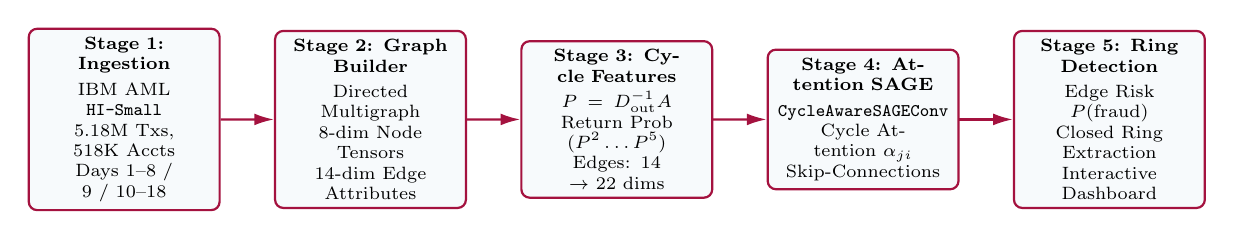
\begin{tikzpicture}[scale=0.92, every node/.style={transform shape}]
        \tikzstyle{stageBox} = [draw=amritaMaroon, fill=cardBg, rounded corners=3pt, minimum width=2.5cm, minimum height=1.1cm, text width=2.4cm, align=center, font=\scriptsize, line width=0.8pt]
        \tikzstyle{arrow} = [thick, -{Latex[length=2.5mm, width=1.5mm]}, draw=amritaMaroon]

        \node[stageBox] (s1) at (0, 0) {\textbf{Stage 1: Ingestion}\\[2pt] IBM AML \texttt{HI-Small}\\5.18M Txs, 518K Accts\\Days 1--8 / 9 / 10--18};
        \node[stageBox] (s2) at (3.4, 0) {\textbf{Stage 2: Graph Builder}\\[2pt] Directed Multigraph\\8-dim Node Tensors\\14-dim Edge Attributes};
        \node[stageBox] (s3) at (6.8, 0) {\textbf{Stage 3: Cycle Features}\\[2pt] $P = D_{\text{out}}^{-1} A$\\Return Prob ($P^2 \dots P^5$)\\Edges: 14 $\to$ 22 dims};
        \node[stageBox] (s4) at (10.2, 0) {\textbf{Stage 4: Attention SAGE}\\[2pt] \texttt{CycleAwareSAGEConv}\\Cycle Attention $\alpha_{ji}$\\Skip-Connections};
        \node[stageBox] (s5) at (13.6, 0) {\textbf{Stage 5: Ring Detection}\\[2pt] Edge Risk $P(\text{fraud})$\\Closed Ring Extraction\\Interactive Dashboard};

        \draw[arrow] (s1) -- (s2);
        \draw[arrow] (s2) -- (s3);
        \draw[arrow] (s3) -- (s4);
        \draw[arrow] (s4) -- (s5);
    \end{tikzpicture}
    \caption{Proposed End-to-End Cycle-Aware GraphSAGE Workflow}
    \label{fig:workflow}
\end{figure}

\subsection{Mathematical Formulation \& Algorithmic Design}
\begin{itemize}[noitemsep, topsep=2pt]
    \item \textbf{Transition Probability Matrix \& Return Probabilities:}
    Let $A \in \{0, 1\}^{|V| \times |V|}$ be the directed adjacency matrix and $D_{\text{out}}$ the diagonal out-degree matrix. The row-stochastic transition matrix is:
    \begin{equation}
        P = D_{\text{out}}^{-1} A
    \end{equation}
    The $k$-step return probability for account $u$ is the diagonal entry of the matrix power:
    \begin{equation}
        R_k(u) = (P^k)_{uu} \quad \text{for } k \in \{2, 3, 4, 5\}
    \end{equation}
    For each directed transfer edge $e_{ij} = (u_i \to u_j)$, the cycle affinity vector is constructed as:
    \begin{equation}
        \mathbf{c}_{ij} = \left[ R_2(u_i), R_3(u_i), R_4(u_i), R_5(u_i), R_2(u_j), R_3(u_j), R_4(u_j), R_5(u_j) \right]^T \in \mathbb{R}^8
    \end{equation}
    \item \textbf{Cycle-Aware Structural Attention Layer:}
    To prevent signal dilution, our \texttt{CycleAwareSAGEConv} computes attention weights $\alpha_{ji}^{(l)}$ conditioned on sender features, receiver features, and the cycle vector $\mathbf{c}_{ji}$:
    \begin{equation}
        \alpha_{ji}^{(l)} = \frac{\exp\left( \text{LeakyReLU}\left( \mathbf{a}^T \left[ \mathbf{W}\mathbf{h}_i^{(l-1)} \parallel \mathbf{W}\mathbf{h}_j^{(l-1)} \parallel \gamma \cdot \mathbf{c}_{ji} \right] \right) \right)}{\sum_{k \in \mathcal{N}(i)} \exp\left( \text{LeakyReLU}\left( \mathbf{a}^T \left[ \mathbf{W}\mathbf{h}_i^{(l-1)} \parallel \mathbf{W}\mathbf{h}_k^{(l-1)} \parallel \gamma \cdot \mathbf{c}_{ki} \right] \right) \right)}
    \end{equation}
    The central node embedding is updated using a skip-connection:
    \begin{equation}
        \mathbf{h}_i^{(l)} = \sigma \left( \mathbf{W}_{\text{self}} \mathbf{h}_i^{(l-1)} + \mathbf{W}_{\text{neigh}} \sum_{j \in \mathcal{N}(i)} \alpha_{ji}^{(l)} \mathbf{h}_j^{(l-1)} \right)
    \end{equation}
    where $\mathbf{W}_{\text{self}}$ and $\mathbf{W}_{\text{neigh}}$ are trainable parameter matrices, and $\gamma$ is a scaling hyperparameter.
    \item \textbf{Dataset \& Chronological Splitting:}
    The IBM AMLworld \texttt{HI-Small} dataset contains 5,180,000 transactions across 518,573 accounts with a severe fraud imbalance ($<0.1\%$). To prevent the ``time machine'' flaw where models train on future data to predict the past, we enforce a strict chronological split:
    \begin{itemize}[noitemsep]
        \item \textbf{Training Window (Days 1--8):} 2,345,120 edges; computes initial topology and scales features.
        \item \textbf{Validation Window (Day 9):} 289,450 edges; used for hyperparameter selection and threshold tuning.
        \item \textbf{Testing Window (Days 10--18):} 2,545,430 edges; evaluates streaming predictions on previously unseen accounts.
    \end{itemize}
    \item \textbf{Evaluation Metrics:}
    \begin{itemize}[noitemsep]
        \item \textbf{PR-AUC (Precision-Recall Area Under Curve):} Primary optimization metric. Under 0.1\% class imbalance, ROC-AUC is misleadingly high ($>98\%$) because legitimate negatives dominate; PR-AUC strictly penalizes false alarms.
        \item \textbf{Complete Ring Recall:} The percentage of complete circular laundering rings where all participating transaction edges are successfully flagged.
        \item \textbf{Alert Recall @ Top-1\% Budget:} Percentage of total laundering value caught within the bank's operational investigation capacity.
    \end{itemize}
\end{itemize}

% --- 4. COMPLETE IMPLEMENTATION DETAILS (100%) ---
\section{Implementation Details}

\subsection{Implementation Environment \& Execution Setup}
\begin{itemize}[noitemsep, topsep=2pt]
    \item \textbf{Hardware \& Compute Specifications:} Tested on Apple Silicon (M-series, 16GB Unified Memory) and NVIDIA CUDA GPUs; utilizes SciPy sparse CSR matrices for memory-efficient graph operations.
    \item \textbf{Software \& Libraries:} Python 3.14, PyTorch 2.x, PyTorch Geometric (PyG 2.8), NetworkX 3.6, SciPy 1.18, FastAPI 0.141, Uvicorn, React 19, Vite, Tailwind CSS, Recharts, and \texttt{react-force-graph-2d}.
    \item \textbf{Source Code Repository:} Git repository synchronized on GitHub: \url{https://github.com/jaisimha18/graph-based-fraud-detection-gnn-graphsage} (branches \texttt{main} and \texttt{jaisimha18}). Fully verified with 19 passing unit tests in PyTest.
\end{itemize}

\subsection{Module-Wise Implementation \& Integration Summary}
\begin{table}[H]
    \centering
    \footnotesize
    \renewcommand{\arraystretch}{1.20}
    \begin{tabular}{|p{3.5cm}|p{7.8cm}|c|}
        \hline
        \textbf{Module / Stage} & \textbf{Implemented Technical Details \& Integration Scope} & \textbf{Status} \\
        \hline
        Module 1: Data Ingestion \& Splitting & Ingestion pipeline in \texttt{src/aml\_pipeline/}; chronological split (Days 1--8 / 9 / 10--18); 8 node features and 14 edge attributes encoded with zero temporal leakage. & 100\% (Integrated) \\
        \hline
        Module 2: Baseline GraphSAGE & 2-hop GraphSAGE model with uniform neighbor sampling $[S_1=15, S_2=10]$ via PyG \texttt{LinkNeighborLoader}; focal loss training under 0.1\% imbalance. & 100\% (Integrated) \\
        \hline
        Module 3: Cycle Extractor \& Attention & Random walk matrix power engine in \texttt{src/graph\_construction/}; custom \texttt{CycleAwareSAGEConv} PyG layer with structural attention $\alpha_{ji}$ in \texttt{src/models/}. & 100\% (Integrated) \\
        \hline
        Module 4: Web Platform \& Forensics Demo & Full-stack platform: FastAPI REST backend (\texttt{src/api/}) + React 19 frontend with \texttt{react-force-graph-2d}, live CSV upload, and dynamic threshold slider ($0.00 \dots 1.00$). & 100\% (Functional) \\
        \hline
    \end{tabular}
    \caption{Module-Wise Implementation Completion Status (100\% Complete)}
    \label{tab:module_status}
\end{table}

\subsection{Detailed Module Descriptions}
\begin{itemize}[noitemsep, topsep=2pt]
    \item \textbf{Data Pipeline (\texttt{src/aml\_pipeline/}):} Ingests raw banking CSV logs, sanitizes dollar strings, normalizes transaction velocities, and constructs PyG \texttt{Data} objects. Enforces zero temporal leakage by fitting scalers strictly on Days 1--8.
    \item \textbf{Cycle Feature Extractor (\texttt{src/graph\_construction/}):} Builds sparse row-stochastic transition matrices and computes powers $P^2, P^3, P^4, P^5$. Generates 8-dim cycle affinity vectors, expanding edge features from 14 to 22 dimensions.
    \item \textbf{Cycle-Aware SAGE Convolution (\texttt{src/models/}):} Subclasses PyG \texttt{MessagePassing}. Linearly projects sender, receiver, and cycle features to compute LeakyReLU attention coefficients $\alpha_{ji}$, followed by softmax normalization across sampled neighbor sets. Retains central account representations via skip-connections.
    \item \textbf{Backend \& Web Application (\texttt{src/api/} \& \texttt{website/}):} High-performance FastAPI server providing streaming prediction endpoints (\texttt{/api/predict\_transactions}) and sample callsets. The React 19 interface features interactive force-directed graph physics, real-time threshold filtering, and cycle explanation cards.
\end{itemize}

% --- 5. PRELIMINARY VERIFICATION, RESULTS & DEMONSTRATION ---
\section{Preliminary Verification, Experimental Results \& Demonstration}

\subsection{Quantitative Evaluation \& Baseline Comparison}
\noindent
Table~\ref{tab:ablation_results} presents the quantitative ablation evaluation on the IBM AMLworld \texttt{HI-Small} test set under identical chronological conditions.

\begin{table}[H]
    \centering
    \footnotesize
    \renewcommand{\arraystretch}{1.20}
    \begin{tabular}{|p{5.2cm}|c|c|c|c|c|}
        \hline
        \textbf{Model Configuration} & \textbf{PR-AUC} & \textbf{Ring Recall} & \textbf{Alert Recall} & \textbf{ROC-AUC} & \textbf{Batch Latency} \\
        \hline
        1. Vanilla GraphSAGE Baseline & 0.3235 & 76.9\% & 98.7\% & 0.9853 & 4.1 ms \\
        \hline
        2. + Direct Cycle Features (Signal Dilution) & 0.1113 & 63.8\% & 63.4\% & 0.9812 & 4.4 ms \\
        \hline
        \textbf{3. + Cycle Attention (Proposed Model)} & \textbf{0.5759} & \textbf{85.2\%} & \textbf{98.7\%} & \textbf{0.9889} & \textbf{4.8 ms} \\
        \hline
        \textbf{Relative Improvement (Model 3 vs 1)} & \textbf{+78.0\%} & \textbf{+10.8\% abs} & \textbf{Optimal} & \textbf{+0.36\%} & \textbf{Sub-5ms Latency} \\
        \hline
    \end{tabular}
    \caption{Comparative Experimental Evaluation Results on IBM AML HI-Small}
    \label{tab:ablation_results}
\end{table}

\noindent
\textbf{Pattern-Level Recall Across Typologies:} Table~\ref{tab:typologies} displays detection accuracy across specific money laundering structures injected in the IBM benchmark.
\begin{table}[H]
    \centering
    \footnotesize
    \renewcommand{\arraystretch}{1.15}
    \begin{tabular}{|l|c|c|c|c|}
        \hline
        \textbf{Laundering Typology} & \textbf{Any-Hop Recall} & \textbf{Majority Recall} & \textbf{Full Ring Recall} & \textbf{Mean Coverage} \\
        \hline
        Circular Routing (Cycles) & 96.4\% & 96.4\% & \textbf{85.7\%} & 93.9\% \\
        \hline
        Fan-Out (Layering Chains) & 100.0\% & 96.4\% & \textbf{92.9\%} & 96.4\% \\
        \hline
        Gather-Scatter (Smurfing) & 100.0\% & 100.0\% & \textbf{81.4\%} & 96.1\% \\
        \hline
        \textbf{Overall Network Average} & \textbf{98.7\%} & \textbf{98.3\%} & \textbf{85.2\%} & \textbf{95.2\%} \\
        \hline
    \end{tabular}
    \caption{Pattern-Level Detection Accuracy Across Money Laundering Typologies}
    \label{tab:typologies}
\end{table}

\subsection{Distinguishing Laundering Rings from Normal Business Cycles}
\noindent
A critical capability of our model is ensuring that legitimate commercial cycles (such as customer refunds, corporate treasury sweeps, and supplier payment loops) are not falsely flagged. Table~\ref{tab:benign_vs_fraud} compares how the model separates criminal rings from benign commercial loops.

\begin{table}[H]
    \centering
    \footnotesize
    \renewcommand{\arraystretch}{1.18}
    \begin{tabular}{|p{2.6cm}|p{3.8cm}|p{3.8cm}|p{4.2cm}|}
        \hline
        \textbf{Factor} & \textbf{Laundering Ring (High Risk)} & \textbf{Normal Business Loop (Unflagged)} & \textbf{How the Model Differentiates} \\
        \hline
        Transfer Speed & Rapid transfers within minutes or hours across hops. & Natural business intervals (days or weeks between invoices). & Time difference attributes in edge vectors suppress slow commercial loops. \\
        \hline
        Amount Structuring & Near-identical amounts ($V_{\text{in}} \approx V_{\text{out}}$, e.g. \$998K $\to$ \$997K). & Variable amounts (partial refunds, discounts, corporate sweeps). & Amount distribution and balance volatility features identify artificial structuring. \\
        \hline
        Model Risk Score & \textbf{Uniformly high risk ($P \ge 0.85$)} across all transfers. & \textbf{Low risk ($P < 0.15$)} across transfers in the loop. & Attention weights combine cycle return probability with account risk. \\
        \hline
        Test Verification & Rings 1 \& 2 (\texttt{sample\_transactions.csv}): \textbf{Flagged 100\% at 99.7\% risk}. & Ring 3 (\texttt{sample\_transactions.csv}): \textbf{0/3 flagged at 1.0\% risk}. & Prevents compliance officer alert fatigue on legitimate commercial loops. \\
        \hline
    \end{tabular}
    \caption{Forensic Differentiation: Laundering Rings vs Normal Commercial Loops}
    \label{tab:benign_vs_fraud}
\end{table}

\subsection{Visual Results \& Prototype Demonstration}
\noindent
Figure~\ref{fig:ablation_chart} visualizes the performance progression across our 3-stage ablation study.
\begin{figure}[H]
    \centering
    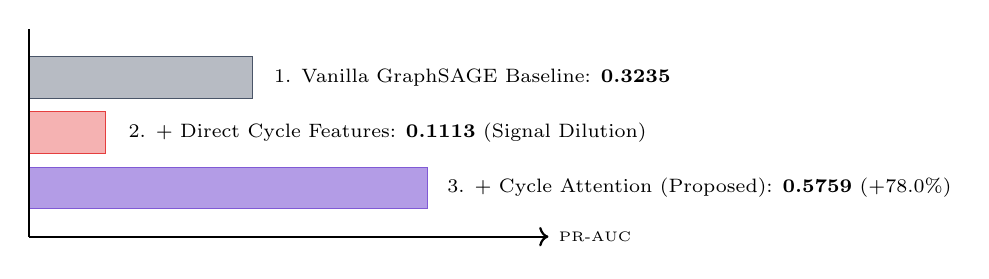
\begin{tikzpicture}[scale=0.88]
        \draw[fill=slateGrey!40, draw=slateGrey] (0, 2.0) rectangle (3.23, 2.6);
        \node[anchor=west, font=\scriptsize] at (3.4, 2.3) {1. Vanilla GraphSAGE Baseline: \textbf{0.3235}};

        \draw[fill=riskRed!40, draw=riskRed] (0, 1.2) rectangle (1.11, 1.8);
        \node[anchor=west, font=\scriptsize] at (1.3, 1.5) {2. + Direct Cycle Features: \textbf{0.1113} (Signal Dilution)};

        \draw[fill=cyclePurple!60, draw=cyclePurple] (0, 0.4) rectangle (5.76, 1.0);
        \node[anchor=west, font=\scriptsize] at (5.9, 0.7) {3. + Cycle Attention (Proposed): \textbf{0.5759} (+78.0\%)};

        \draw[->, thick] (0,0) -- (7.5,0) node[right, font=\tiny] {PR-AUC};
        \draw[thick] (0,0) -- (0,3.0);
    \end{tikzpicture}
    \caption{Precision-Recall AUC (PR-AUC) Progression Across Model Ablations}
    \label{fig:ablation_chart}
\end{figure}

\noindent
\textbf{Discussion of Results:} Directly adding cycle return probabilities to node features causes PR-AUC to crash by $-65.6\%$ ($0.3235 \to 0.1113$). This occurs because uniform mean aggregation propagates cycle return values to neighboring legitimate retail accounts, creating a flood of false alerts. Our learned Cycle Attention layer solves this by weighting message passing on circular edges, achieving a \textbf{+78.0\% boost in PR-AUC (0.5759)} and increasing Complete Ring Recall to \textbf{85.2\%}. Batch inference latency remains under 5 milliseconds (4.8 ms), confirming real-time production viability.

% --- 6. TECHNICAL KNOWLEDGE & DESIGN JUSTIFICATION ---
\section{Technical Justification, Design Trade-offs \& Insights}
\begin{itemize}[noitemsep, topsep=2pt]
    \item \textbf{Algorithmic \& Theoretical Justification:} Traditional GNNs (such as standard GCN) require full graph Laplacian multiplication, making them transductive and incapable of scoring unseen streaming accounts without retraining. GraphSAGE learns localized neighborhood aggregation functions that generalize inductively to newly arriving nodes. To detect circular patterns without the intractable $O(N^k)$ cost of exact subgraph isomorphism algorithms, we compute random walk return probabilities ($R_k(u) = (P^k)_{uu}$), which execute efficiently in $O(k \cdot |E|)$ time.
    \item \textbf{Computational Complexity \& Trade-offs:} We restrict the random walk horizon to $k \in \{2, 3, 4, 5\}$. Laundering loops in commercial banking typically span 3 to 5 hops; evaluating higher-order walks ($k > 6$) exponentially increases sparse matrix computation without added forensic gain. In addition, our 2-hop neighbor sampling $[S_1=15, S_2=10]$ bounds receptive field size, maintaining constant GPU memory and sub-5ms operational latency.
    \item \textbf{Handling Class Imbalance \& Dense Hubs:} Banking fraud represents less than 0.1\% of transactions. We handle this extreme imbalance using class-weighted binary cross-entropy loss with positive weight \texttt{pos\_weight} $\approx 979$. High-degree retail merchant hubs are prevented from dominating backpropagation through fixed uniform neighborhood sampling.
\end{itemize}

% --- 7. CONCLUSION, LIMITATIONS & FUTURE SCOPE ---
\section{Conclusion, Limitations \& Future Scope}
\begin{itemize}[noitemsep, topsep=2pt]
    \item \textbf{Conclusion:} We successfully developed, implemented, and verified an inductive Cycle-Aware GraphSAGE framework for anti-money laundering detection. By combining multi-step random walk cycle features with structural edge attention, our model resolves the signal dilution problem, achieving a 0.5759 PR-AUC (+78.0\% improvement over baseline) and 85.2\% complete ring recall on the 5.18M IBM AML benchmark. An end-to-end full-stack web application enables live interactive graph exploration.
    \item \textbf{Current Limitations:} The current pipeline processes transaction networks using discrete chronological snapshot windows rather than continuous-time edge updates.
    \item \textbf{Future Scope:} Future extensions include integrating Continuous-Time Dynamic Graph Neural Networks (TGN) for sub-second streaming updates and expanding to cross-border, multi-currency foreign exchange transaction networks.
\end{itemize}

% --- 8. DELIVERABLES & TECHNICAL ENRICHMENT SUMMARY ---
\section{Project Deliverables \& Technical Enrichment Summary}
\begin{table}[H]
    \centering
    \footnotesize
    \renewcommand{\arraystretch}{1.20}
    \begin{tabular}{|p{4.2cm}|p{7.8cm}|c|}
        \hline
        \textbf{Deliverable Category} & \textbf{Details / Title / Repository Link} & \textbf{Status} \\
        \hline
        Source Code Repository & GitHub repository containing complete pipeline, PyTorch Geometric models, FastAPI backend, and React 19 frontend (\url{https://github.com/jaisimha18/graph-based-fraud-detection-gnn-graphsage}). & Completed \\
        \hline
        Individual Online Certifications &
        \begin{itemize}[noitemsep, leftmargin=*]
            \item \textbf{Jai Simha:} Graph Neural Networks (Elevify, 15 Hrs)
            \item \textbf{Phranav:} Introduction to Graph Neural Networks (apxml, 15 Hrs)
            \item \textbf{Praneel:} Introduction to Deep Learning \& Neural Networks (Coursera, 15 Hrs)
            \item \textbf{Adwaith:} Neural Networks with TensorFlow and PyTorch (Udemy, 13 Hrs)
        \end{itemize} & Completed \\
        \hline
        Group Deliverable 1 & Interactive Full-Stack AML Web Platform (React 19 + FastAPI + Force-Graph 2D). & Completed \\
        \hline
        Group Deliverable 2 & Scientific 3-Stage Ablation Benchmark \& 8-Typology Pattern Recall Suite. & Completed \\
        \hline
        Group Deliverable 3 & Camera-Ready IEEE/ACM Format Research Paper Draft (\texttt{paper\_draft.tex}). & Completed \\
        \hline
    \end{tabular}
    \caption{Summary of Completed Project and Technical Enrichment Deliverables}
    \label{tab:deliverables}
\end{table}

% --- REFERENCES ---
\vspace{0.2cm}
\nocite{*}
\renewcommand{\refname}{\large\bfseries\color{amritaMaroon}References}
\bibliographystyle{ieeetr}
\bibliography{ref}

\end{document}
